\documentclass[t, screen, aspectratio=43]{beamer}
\usepackage[T1]{fontenc}
\usepackage[utf8]{inputenc}
\usepackage{epsf}
\usepackage{graphicx}
\usepackage{geometry}
\usepackage{tabularx}
\usepackage[table]{colortbl}
\usepackage{xcolor}
\usepackage{soul}
\usepackage[normalem]{ulem}
\usepackage{tikz}
\usepackage{subcaption}
% Use the NTNU-temaet for beamer 
% \usetheme[style=ntnu|simple|vertical|horizontal, 
%     language=bm|nn|en, 
%     smalltitle, 
%     city=all|trondheim|alesund|gjovik]{ntnu2017}
\usetheme[style=helvet,language=en]{ntnu2017}

\usepackage[english]{babel}
\usepackage[style=numeric,backend=biber,natbib=false,sorting=none]{biblatex}

\title[Short title]{Ultra low power integer-N ADPLL}
\subtitle{Master's thesis project - meeting 3}
\author[C Nielsen]{Cole Nielsen}
\institute[NTNU]{Department of Electronic Systems, NTNU}
\date{31 January 2020 (calendar week 5)}
%\date{} % To have an empty date

\addbibresource{example.bib} % Add bibliography database

% Set the reference style to numeric.
% See here: http://tex.stackexchange.com/questions/68080/beamer-bibliography-icon
\setbeamertemplate{bibliography item}[text] 

% Set bibliography fonts to a small size.
\renewcommand*{\bibfont}{\footnotesize}

\usepackage{tikz}
\usepackage{enumitem}
\newcommand*\mycirc[1]{%
\begin{tikzpicture}[baseline=(C.base)]
	\node[draw,circle,inner sep=1pt,minimum size=3ex](C){#1};
\end{tikzpicture}}


\begin{document}

\begin{frame}
	\titlepage%
\end{frame}

% Alternatively, special title page command to get a different background
% \ntnutitlepage

% #############################################################################
% This week
% #############################################################################

\begin{frame}
	\frametitle{Overview}
	\begin{block}{For this week...}
		\begin{enumerate}[itemsep=4pt,label=\protect\mycirc{\arabic*}]
			\scriptsize
			\item Estimation of loop filter logic power.
			\item Criteria to push envelope versus state of art.
			\item Ideal Virtuoso PLL setup with Verilog(-ams) models of components.
		\end{enumerate} 
	\end{block}	
\end{frame}


% #############################################################################
% This week
% #############################################################################


% #############################################################################
% Physical limits
% #############################################################################

\begin{frame}
	\frametitle{Digital loop filter power estimate.}
	\begin{block}{Assumptions}
		\begin{itemize}[itemsep=4pt,label=\protect---]
			\scriptsize
			\item Arising from \textit{paranoia} about digital loop filter power consumption (target < 10$\mu$W).
			\item Estimate equivalent number ($\textrm{N}_{\mathrm{NAND2}}$) of NAND2 gates for (a) 4x N-bit Baugh-Wooley array multipliers, (b) 3x N-bit Brent-Kung tree adders. Also, account for DFFs ($\textrm{N}_{\mathrm{DFF}}$) in 3x N-bit registers.
			\item Assume $\textrm{E}_{op}$ = 1 fJ per NAND2 or DFF operation. Stian Østerhus' thesis from 2018 with 22-FDX found 139.37-239.42 aJ/operation for NAND, and 396.91-418.27 aJ/operation for DFF depending on with/without body bias with 0.35V supply (post layout).
			\item Activity factor $\alpha$ of loop filter logic is uncertain... In steady state (BB-PD feedback), loop filter input will change by ca. 1 LSB per cycle so I expect $\alpha$ is low.
		\end{itemize} 
		\footnotesize
		\begin{equation}
			\textrm{P}_{logic} = \alpha (\textrm{N}_{\mathrm{NAND2}}+\textrm{N}_{\mathrm{DFF}})\textrm{E}_{op}f_{clk}
		\end{equation}
		\tiny
		\hspace{2em}\vspace{1em}\textbf{Note: Only considering dynamic power here.}
	\end{block}	
\end{frame}

\begin{frame}
	\frametitle{Digital loop filter power estimate.}
	\begin{block}{Component-level specs}
		\scriptsize
		\begin{itemize}[itemsep=4pt,label=\protect---]
			\scriptsize
			\item Given 22-FDX yields ca. 5.5 MGates/mm$^2$, assume $\alpha$ = 0.1, $f_{clk}$ = 16 MHz:
		\end{itemize} 
	\vspace{-1em}
	\begin{table}[h!]
		\centering
		\def\arraystretch{1.5}		
		\setlength\arrayrulewidth{0.75pt}
		\setlength{\tabcolsep}{1em} % for the horizontal padding
		\tiny
		\begin{tabular}{|c|c|c|c|c|}
			\hline 
			\rule[-1ex]{0pt}{2.5ex} \cellcolor{gray!40}\textbf{Datapath bits} & \cellcolor{gray!40}\textbf{Gates+DFFs} & \cellcolor{gray!40}\textbf{Area} [$\mu m^2$] & \cellcolor{gray!40}\textbf{Square side [$\mu m$]} &  \cellcolor{gray!40}\textbf{Power} [$\mu$W], $\alpha$ = 0.1\\ 
			\hline 
			\rule[-1ex]{0pt}{2.5ex} 8 & 2652 & 521 & 22.8 & 4.24 \\ 
			\hline 
			\rule[-1ex]{0pt}{2.5ex} 9 & 3390 & 660 & 25.7 & 5.42 \\ 
			\hline 
			\rule[-1ex]{0pt}{2.5ex} 10 & 4213 & 815 & 28.5 & 6.74 \\ 
			\hline 
			\rule[-1ex]{0pt}{2.5ex} 11 & 5127 & 986 & 31.4 & 8.20 \\ 
			\hline 
			\rule[-1ex]{0pt}{2.5ex} 12 & 6126 & 1172 & 34.2 & 9.80 \\ 
			\hline 
			\rule[-1ex]{0pt}{2.5ex} 13 & 7216 & 1375 & 37.1 & 11.5 \\ 
			\hline 
			\rule[-1ex]{0pt}{2.5ex} 14 & 8391 & 1594& 39.9 & 13.4 \\ 
			\hline 
			\rule[-1ex]{0pt}{2.5ex} 15 & 9657 & 1829 & 42.8 & 15.5 \\ 
			\hline 
			\rule[-1ex]{0pt}{2.5ex} 16 & 11008 & 2080 & 45.6 & 17.6 \\ 
			\hline 
		\end{tabular} 
		% \caption{Assigned specifications for branch line hybrid design.}
		% \label{asgn_specs}
		\label{design_specs}
	\end{table}   
		\scriptsize
		\vspace{-1em}
		\begin{itemize}[itemsep=4pt,label=\protect---]
			\scriptsize
			\item Power in line with the naive 10$\mu$W goal. May require low supply V$_{DD}$, however.
			\item Logic under 50 $\mu$m x 50 $\mu$m. \textbf{Target whole PLL under 100 $\mu$m x 100 $\mu$m (0.01 mm$^2$??}
		\end{itemize} 
	\end{block}    
\end{frame}

\begin{frame}
	\frametitle{Pushing performance envelope.}
	\begin{block}{State of art}
	\begin{minipage}{5.5cm}
	\tiny\vspace{0.5em}
		\hspace{1em}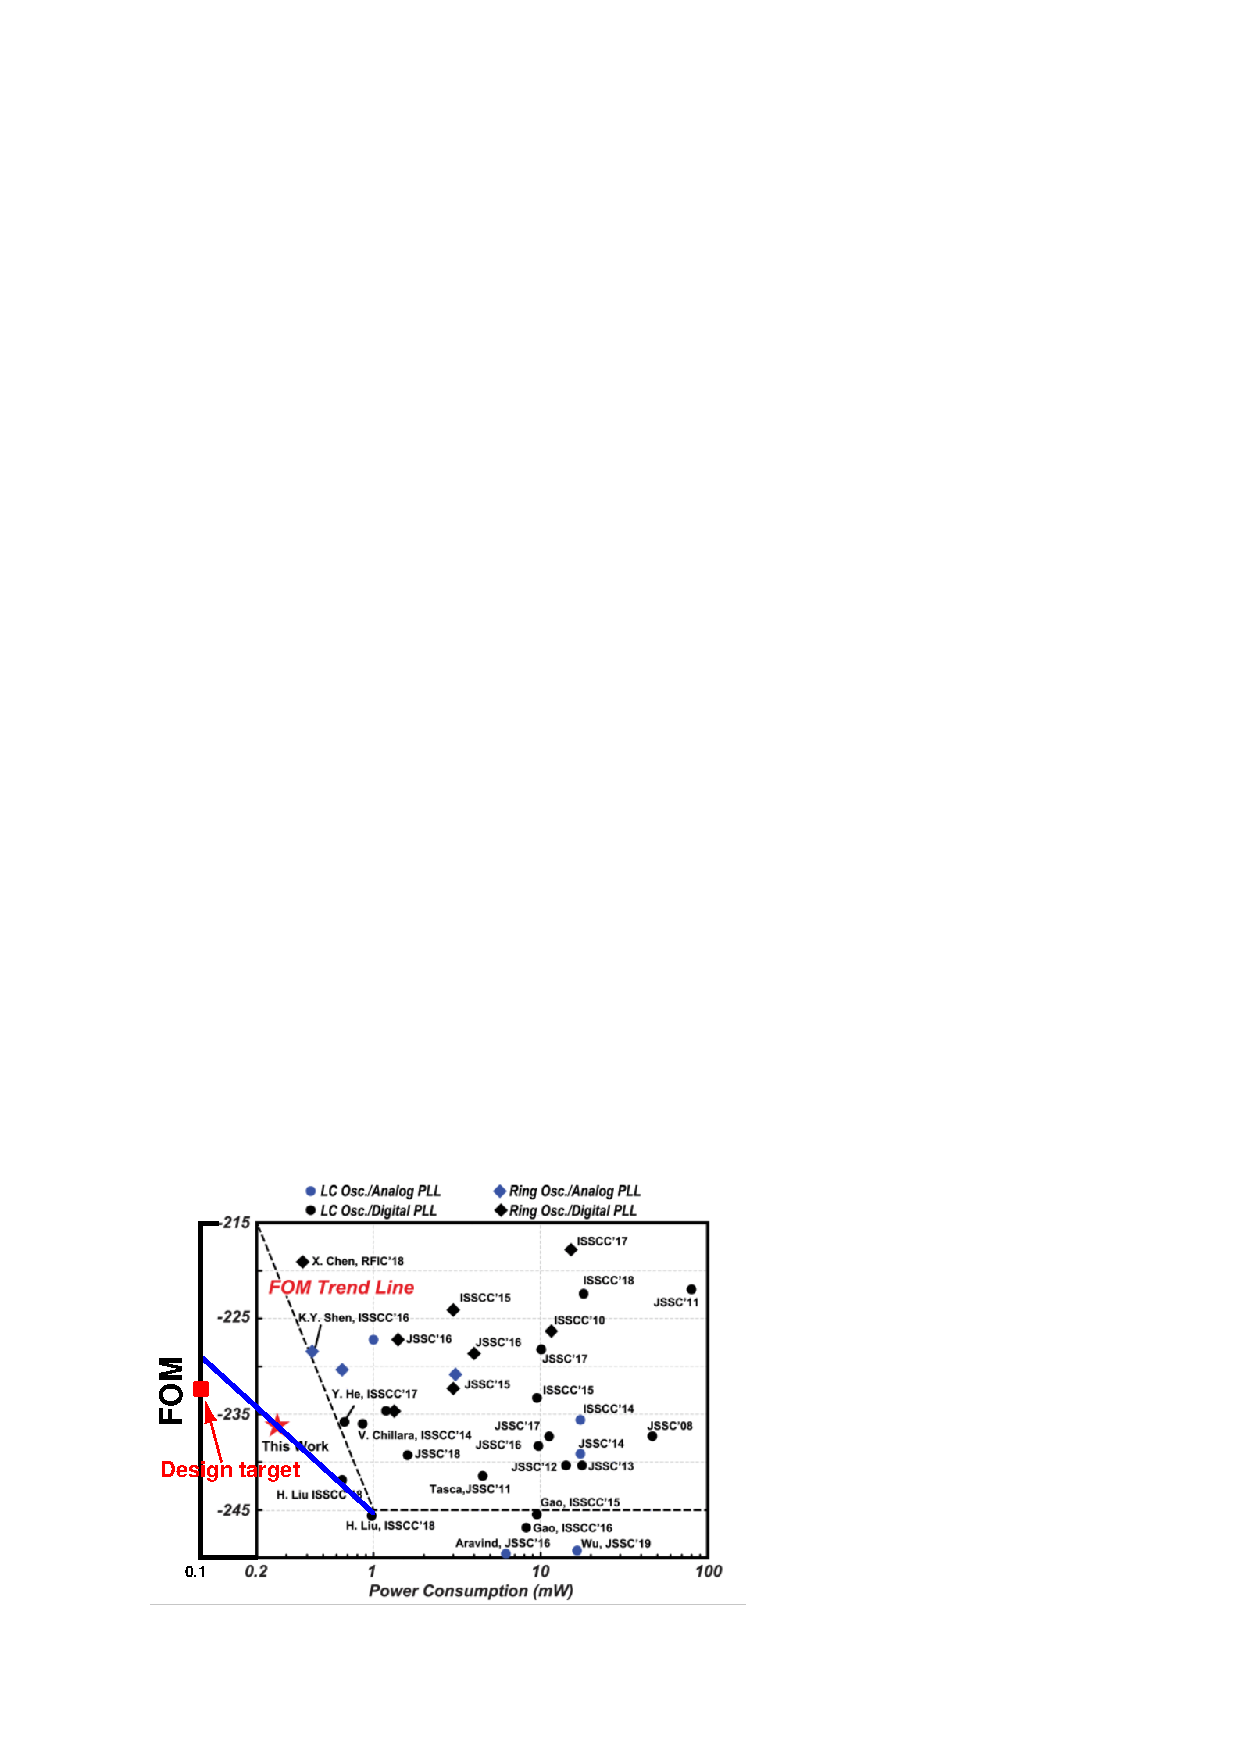
\includegraphics[width=1\textwidth, angle=0]{power_fom_state_art.pdf}
		\tiny
		Figure from 2019 JSSC paper [1].
		\tiny\vspace{-1em}
		\begin{equation}
			\textnormal{FOM}_{\textnormal{jitter}} = 10 \log_{10}\left(\left(\frac{\sigma_{t_{jitter}}}{\textrm{1 s}}\right)^2\cdot\frac{\textnormal{P}}{\textnormal{1 mW}}\right)
		\end{equation}
		{If CNR = 20 dBc @ 2.4GHz $\rightarrow$ $\sigma_{t_{jitter}}$ = 6.5 ps $\rightarrow$ FOM = -233 dB.}
	\end{minipage}
	\begin{minipage}{5.5cm}
		\hspace{1em}\includegraphics[width=1\textwidth, angle=0]{fom_area_state_art.pdf}
		\tiny
		\begin{itemize}[itemsep=4pt,label=\protect---]
			\item Figure from 2018 JSSC paper [2].
			\item FOM$_r$ is with normalization to a 200 MHz reference oscillator. The PLL target for this project translates to FOM$_r$ =-245 dB with a 16 MHz reference.
			\item \textbf{If phase noise can be maintaied with CNR $>$ 20 dBc, and PLL size $<$ 0.01 mm$^2$, design will be state of art.}
		\end{itemize} 	
	\end{minipage}

	\end{block}
\end{frame}

\begin{frame}
	\frametitle{Pushing performance envelope.}
	\begin{block}{Ultra-state of art for size (5 nm)}
		\scriptsize
		\begin{itemize}[itemsep=4pt,label=\protect---]
			\item This is from a sythesized PLL in TSMC 5nm FinFET [3], that \textit{has} been fabricated. The paper is an early release from SSCL. Area is 0.0036 mm$^2$, or 50 $\mu$m x 72 $\mu$m.
			\item Targeting $\textnormal{FOM}_{\textnormal{jitter}} \approx$ -233 dB and < 0.01 mm$^2$ is fairly competitive with the 5nm design.
			\item Paper claims ring oscillator jitter degrades in sub-20nm regime, so 22-FDX may be very advantageous from an analog perspective.
		\end{itemize} 	
		\vspace{-1em}
		\center\includegraphics[width=0.6\textwidth, angle=0]{5nm_pll_perf.png}
	\end{block}
\end{frame}

\begin{frame}
	\frametitle{Pushing performance envelope.}
	\begin{block}{}
		\scriptsize
		To be competitive versus current state of art the following design constraints are being imposed:
		\begin{table}[h!]
			\centering
			\def\arraystretch{1.5}		
			\setlength\arrayrulewidth{0.75pt}
			\setlength{\tabcolsep}{1em} % for the horizontal padding
			\begin{tabular}{|l|r|l|}
				\hline 
				\rule[-1ex]{0pt}{2.5ex} \cellcolor{gray!40}\textbf{Parameter} & \cellcolor{gray!40}\textbf{Value} & \cellcolor{gray!40}\textbf{Unit }\\ 
				\hline 
				\rule[-1ex]{0pt}{2.5ex} \textbf{CNR}  & $\geq$ 16.5 & dBc \\ 
				\hline 
				\rule[-1ex]{0pt}{2.5ex} \textbf{FOM}$_{\textnormal{jitter}}$ & $\leq$ -230 & dB \\ 
				\hline 
				\rule[-1ex]{0pt}{2.5ex} \textbf{Power} & $\leq$ 100  &$\mu$W \\ 
				\hline 
				\rule[-1ex]{0pt}{2.5ex} \textbf{Area} & $<$ 0.01  & mm$^2$ \\ 
				\hline 
			\end{tabular} 
			% \caption{Assigned specifications for branch line hybrid design.}
			% \label{asgn_specs}
		\end{table}   
	\end{block}    
\end{frame}

\begin{frame}
	\frametitle{Ideal PLL Testbench in Virtuoso}
	\begin{block}{Verilog(-AMS) Models}
	\begin{minipage}{5cm}
		\begin{itemize}[itemsep=4pt,label=\protect---]
			\scriptsize
			\item Wrote Verilog models for BB-PD, divider, loop filter. Wrote Verilog-AMS models for oscillator and TDC.
			\item Issue with Verilog-AMS: missing executable for xmvlog compiler? 
		\end{itemize} 	
	\end{minipage}
	\begin{minipage}{6cm}
		\vspace{1em}
		\hspace{1em}\includegraphics[width=1\textwidth, angle=0]{xmvlog.png}
	\end{minipage}
	\end{block}
\end{frame}


% #############################################################################
% Loop Dynamics (continuous)
% #############################################################################

% \begin{frame}
% 	\frametitle{Loop Dynamics}
% 	\begin{block}{Still To Do}
% 		\vspace{-.2em}
% 		\begin{itemize}
% 			\footnotesize
% 			\item Standard approach to used mixed continuous/discrete time mathematical model for DPLL. 
% 			\item Plot of RO phase noise (typical)
% 			\item Automatic analysis of performance (lock detection, residual phase modulation, lock-in/pull-in range).
% 			\item Automatic optimization (using gradient descent) of PLL parameters?
% 			\item Z-domain modeling of loop? Develop (by hand) some ideal transfer funtions for loop.

% 		\end{itemize}    
% 	\end{block}
% \end{frame}

% #############################################################################
% Architecture - block diagram
% #############################################################################


\begin{frame}
	\frametitle{Architecture}
	\begin{block}{Block Diagram}
	\center\includegraphics[width=0.8\textwidth, angle=0]{pll_master_arch.pdf}

	\end{block}
		\begin{block}{Power Targets}
		\vspace{-.1em}
		\begin{table}[htb!]
			\tiny
			\centering
			\def\arraystretch{1.5}		
			\setlength\arrayrulewidth{0.75pt}
			\setlength{\tabcolsep}{1em} % for the horizontal padding
			\begin{tabular}{|l|l|l|l|l|l|}
				\hline 
				\rule[-1ex]{0pt}{2.5ex} \cellcolor{gray!40}\textbf{DCO} & \cellcolor{gray!40}\textbf{Phase detector} & \cellcolor{gray!40}\textbf{Divider }& \cellcolor{gray!40}\textbf{Digital (LF)}& \cellcolor{gray!40}\textbf{Other} & \cellcolor{gray!40}\textbf{SUM} \\ 
				\hline 
				\rule[-1ex]{0pt}{2.5ex} 50 $\mu$W& 10 $\mu$W & 10 $\mu$W & 10 $\mu$W  & $<<$ 10 $\mu$W & $<$ 100 $\mu$W\\ 
				\hline 
			\end{tabular} 
			% \caption{Assigned specifications for branch line hybrid design.}
			% \label{asgn_specs}
		\end{table}   
	\end{block}

\end{frame}

% #############################################################################
% Specification
% #############################################################################

\begin{frame}
	\frametitle{Specification\color{black}}
	\begin{block}{System Performance Targets}
		\tiny
		\begin{table}[h!]
			\centering
			\def\arraystretch{1.5}		
			\setlength\arrayrulewidth{0.75pt}
			\setlength{\tabcolsep}{1em} % for the horizontal padding
			\begin{tabular}{|l|r|l|l|}
				\hline 
				\rule[-1ex]{0pt}{2.5ex} \cellcolor{gray!40}\textbf{Parameter} & \cellcolor{gray!40}\textbf{Value} & \cellcolor{gray!40}\textbf{Unit }& \cellcolor{gray!40}\textbf{Notes}\\ 
				\hline 
				\rule[-1ex]{0pt}{2.5ex} \textbf{Frequency}  & 2.4-2.4835 & GHz & 2.4G ISM Band\\ 
				\hline 
				\rule[-1ex]{0pt}{2.5ex} \textbf{Ref. frequency} & 16 & MHz & Yields 6 channels \\ 
				\hline 
				\rule[-1ex]{0pt}{2.5ex} \textbf{Power} & $\leq$ 100  &$\mu$W & minimize!\\ 
				\hline 
				\rule[-1ex]{0pt}{2.5ex} \textbf{FSK BER} & $\leq$ 1e-2  & & GFSK\textbf{*} with $f_{dev}$=$\pm$250 KHz\\ 
				\hline 
				\rule[-1ex]{0pt}{2.5ex} \textbf{CNR} & $>$ 16.5 & dBc&Yields -233 dB FOM$_{jitter}$ \\ 
				\hline 
				\rule[-1ex]{0pt}{2.5ex} \textbf{Initial Lock Time} & $\leq$ 10 & $\mu$s & Upon cold start \\ 
				\hline 
				\rule[-1ex]{0pt}{2.5ex} \textbf{Re-lock Time} & $\leq$ 5 & $\mu$s & Coming out of standby \\ 
				\hline 
				\rule[-1ex]{0pt}{2.5ex} \textbf{Lock $\Delta f$ tolerance} & $10^5$ & Hz& \\ 
				\hline 
				\rule[-1ex]{0pt}{2.5ex} \textbf{FOM}$_{\textnormal{jitter}}$ & $\leq$ -230 & dB & \\ 
				\hline 
				\rule[-1ex]{0pt}{2.5ex} \textbf{Area} & $<$ 0.01  & mm$^2$ & \\ 
				\hline 
			\end{tabular} 
			% \caption{Assigned specifications for branch line hybrid design.}
			% \label{asgn_specs}
		\end{table}   
		\textbf{*} Using BT=0.3, 1 MSymbols/s, 4 demodulated symbols averaged per bit to yield 250 kbps.
	\end{block}    
\end{frame}



\begin{frame}
	\frametitle{Specification\color{black}}
	\begin{block}{Component-level specs}
		\scriptsize
	\begin{table}[h!]
		\centering
		\def\arraystretch{1.5}		
		\setlength\arrayrulewidth{0.75pt}
		\setlength{\tabcolsep}{1em} % for the horizontal padding
		\begin{tabular}{|l|r|l|}
			\hline 
			\rule[-1ex]{0pt}{2.5ex} \cellcolor{gray!40}\textbf{Parameter} & \cellcolor{gray!40}\textbf{Value} & \cellcolor{gray!40}\textbf{Unit }\\ 
			\hline 
			\rule[-1ex]{0pt}{2.5ex} \textbf{Counter range}  & 256 steps & coverage of 150-155 \\ 
			\hline 
			\rule[-1ex]{0pt}{2.5ex} \textbf{Divider ratio} & 150-155  & (For non-counter based)\\ 
			\hline 
			\rule[-1ex]{0pt}{2.5ex} \textbf{TDC resolution} &$\geq$ 155  & steps/reference cycle\\ 
			\hline 
			\rule[-1ex]{0pt}{2.5ex} \textbf{DCO gain $K_{DCO}$} & $10^4$ & Hz/LSB \\ 
			\hline 
			\rule[-1ex]{0pt}{2.5ex} \textbf{DCO Phase noise} &$<$ -80 & dBc/Hz at $\Delta f=10^6$ Hz \\ 
			\hline 
			\rule[-1ex]{0pt}{2.5ex} \textbf{DCO Power} & $\leq$ 50 & $\mu$W \\ 
			\hline 
			\rule[-1ex]{0pt}{2.5ex} \textbf{Digital filter word resolution} & $\leq$ 16 & bits \\ 
			\hline 
		\end{tabular} 
		% \caption{Assigned specifications for branch line hybrid design.}
		% \label{asgn_specs}
		\caption{System-level specifications}
		\label{design_specs}
	\end{table}   
	\end{block}    
\end{frame}

% #############################################################################
% Timeline
% #############################################################################

\begin{frame}
	\frametitle{Time plan (pt. 1)}
	\begin{table}[htb!]
		\tiny
		\centering
		\vspace{-1em}
		\def\arraystretch{1.5}		
		\setlength\arrayrulewidth{0.75pt}
		\setlength{\tabcolsep}{1em} % for the horizontal padding
		\begin{tabular}{|c|l|l|l|}
			\hline 
			\rule[-1ex]{0pt}{2.5ex}\cellcolor{gray!40}\textbf{Week \#} & \cellcolor{gray!40}\textbf{Dates} &\cellcolor{gray!40}\textbf{Tasks} & \cellcolor{gray!40}\textbf{Outcomes}\\ 
			\hline 
			% \rule[-1ex]{0pt}{2.5ex} \cellcolor{green!20}\textbf{3}&\cellcolor{green!20}13.1 - 19.1 &\cellcolor{green!20}Review PLL Design &\cellcolor{green!20}Refreshed Knowledge\\ 
			% \hline 
			\rule[-1ex]{0pt}{2.5ex}\cellcolor{red!40}\textbf{4}&\cellcolor{red!40}20.1 - 26.1 &\cellcolor{red!40}Finalize high level modeling &\cellcolor{red!40}Component level specification\\ 
			\hline 
			\rule[-1ex]{0pt}{2.5ex}\textbf{5}\cellcolor{green!40}&\cellcolor{green!40}27.1 - 2.2 &\cellcolor{green!40}Establish test bench in Virtuoso &\cellcolor{green!40}With ideal PLL implementation\\ 
			\hline 
			\rule[-1ex]{0pt}{2.5ex}\textbf{6}& 3.2 - 9.2& Schem. design: phase detector & TDC - flash and counter based \\ 
			\hline 
			\rule[-1ex]{0pt}{2.5ex}\textbf{7}& 10.2 - 16.2& Schem. design: phase detector & Bang-bang phase detector\\ 
			\hline 
			\rule[-1ex]{0pt}{2.5ex}\textbf{8}&17.2 - 23.2& RTL, synthesis, place\&route & Digital loop filter\\ 
			\hline 
			\rule[-1ex]{0pt}{2.5ex}\textbf{9}&24.2 - 1.3& RTL, synthesis, place\&route & Digital loop filter\\ 
			\hline 
			\rule[-1ex]{0pt}{2.5ex}\textbf{10}&2.3 - 8.3& Schem. design: oscillator & Ring DCO\\ 
			\hline 
			\rule[-1ex]{0pt}{2.5ex}\textbf{11}&9.3 - 15.3& Schem. design: oscillator & LC DCO\\ 
			\hline 
			\rule[-1ex]{0pt}{2.5ex}\textbf{12}&16.3 - 22.3& Schem. design: divider  &TSPC + pulse swallow or sync counter?\\ 
			\hline 
			\rule[-1ex]{0pt}{2.5ex}\textbf{13}&23.3 - 29.3&Schem. design: Calibration& RTL/schem. for calibration\\ 
			\hline 
			\rule[-1ex]{0pt}{2.5ex}\textbf{14}& 30.3 - 5.4 &  Flex week - schem. design & Finalize schematic level design\\ 
			\hline 
			\rule[-1ex]{0pt}{2.5ex}\textbf{15}& 6.4 - 12.4& {\color{red}\textbf{Easter}} & - \\ 
			\hline 
			\rule[-1ex]{0pt}{2.5ex}\textbf{16}& 13.4 - 19.4& Layout & Phase detector\\ 
			\hline 
			\rule[-1ex]{0pt}{2.5ex}\textbf{17}& 20.4 - 26.4& Layout & Oscillator\\ 
			\hline 
		\end{tabular}
		\begin{flushleft}\textbf{Legend:} \colorbox{red!20}{\textbf{Done}} \colorbox{green!20}{\textbf{Current}}  \colorbox{blue!20}{\textbf{Revised}}
		% *I will write the report simultaneously with the work.
		\end{flushleft}
		% \caption{Assigned specifications for branch line hybrid design.}
		% \label{asgn_specs}
	\end{table}   
\end{frame}

\begin{frame}
	\frametitle{Time plan (pt. 2)}
	\begin{table}[htb!]
		\tiny
		\centering
		\vspace{-1em}
		\def\arraystretch{1.5}		
		\setlength\arrayrulewidth{0.75pt}
		\setlength{\tabcolsep}{1em} % for the horizontal padding
		\begin{tabular}{|c|l|l|l|}
			\hline 
			\rule[-1ex]{0pt}{2.5ex}\cellcolor{gray!40}\textbf{Week \#} & \cellcolor{gray!40}\textbf{Dates} &\cellcolor{gray!40}\textbf{Tasks} & \cellcolor{gray!40}\textbf{Outcomes}\\ 
			\hline 
			\rule[-1ex]{0pt}{2.5ex}\textbf{18}& 27.4 - 3.5 & Layout & Divider/calibration\\ 
			\hline 
			\rule[-1ex]{0pt}{2.5ex}\textbf{19}& 4.5 - 10.5 & Layout & Finalization/system integration\\ 
			\hline 
			\rule[-1ex]{0pt}{2.5ex}\textbf{20}& 11.5 - 17.5 & Flex week (layout) OR yield improvement & Depending on progress\\ 
			\hline 
			\rule[-1ex]{0pt}{2.5ex}\textbf{21}& 18.5 - 24.5& {\color{blue}\textbf{Report writing}} & \\ 
			\hline 
			\rule[-1ex]{0pt}{2.5ex}\textbf{22}& 25.5 - 31.5& {\color{blue}\textbf{Report writing}} & \\ 
			\hline 
			\rule[-1ex]{0pt}{2.5ex}\textbf{23}& 1.6 - 7.6& {\color{blue}\textbf{Report writing}} & {\color{red}\textbf{Deadline 8.6}}\\ 
			\hline 
		\end{tabular}
		\begin{flushleft}\textbf{Legend:} \colorbox{red!20}{\textbf{Done}} \colorbox{green!20}{\textbf{Current}}  \colorbox{blue!20}{\textbf{Revised}}
		% *I will write the report simultaneously with the work.
		\end{flushleft}
		% \caption{Assigned specifications for branch line hybrid design.}
		% \label{asgn_specs}
	\end{table}   
\end{frame}


% #############################################################################
% project phases
% #############################################################################

% ############################################################################b#
% References
% #############################################################################


\begin{frame}
	\frametitle{References}
		\scriptsize
		[1]  Liu, H., Shirane, A., Okada, K., Sun, Z., Huang, H., Deng, W., Siriburanon, T., Pang, J., Wang, Y., Wu, R. and Someya, T. (2019). A 265-$\mu$ W Fractional-${N}$ Digital PLL With Seamless Automatic Switching Sub-Sampling/Sampling Feedback Path and Duty-Cycled Frequency-Locked Loop in 65-nm CMOS. IEEE Journal of Solid-State Circuits, 54(12), pp.3478-3492.\par
		\vspace{0.5em}
		[2] Yang, S., Yin, J., Mak, P. and Martins, R. (2019). A 0.0056-mm2 -249-dB-FoM All-Digital MDLL Using a Block-Sharing Offset-Free Frequency-Tracking Loop and Dual Multiplexed-Ring VCOs. IEEE Journal of Solid-State Circuits, 54(1), pp.88-98.\par
		\vspace{0.5em}
		[3] Liu, B., Li, Z., Fu, X., Shirane, A., Kurosu, H., Nakane, Y., Masaki, S., Okada, K., Zhang, Y., Qiu, J., Huang, H., Sun, Z., Xu, D., Zhang, H., Wang, Y. and Pang, J. (2020). A Fully-Synthesizable Fractional-N Injection-Locked PLL for Digital Clocking with Triangle/Sawtooth Spread-Spectrum Modulation Capability in 5 nm CMOS. IEEE Solid-State Circuits Letters, pp.1-1.
	% Navid et al. 2005
\end{frame}


\end{document}
